%!TEX TS-program = xelatex

% Шаблон документа LaTeX создан в 2018 году
% Алексеем Подчезерцевым
% В качестве исходных использованы шаблоны
% 	Данилом Фёдоровых (danil@fedorovykh.ru) 
%		https://www.writelatex.com/coursera/latex/5.2.2
%	LaTeX-шаблон для русской кандидатской диссертации и её автореферата.
%		https://github.com/AndreyAkinshin/Russian-Phd-LaTeX-Dissertation-Template

\documentclass[a4paper,14pt]{article}


%%% Работа с русским языком
\usepackage[english,russian]{babel}   %% загружает пакет многоязыковой вёрстки
\usepackage{fontspec}      %% подготавливает загрузку шрифтов Open Type, True Type и др.
\defaultfontfeatures{Ligatures={TeX},Renderer=Basic}  %% свойства шрифтов по умолчанию
\setmainfont[Ligatures={TeX,Historic}]{Times New Roman} %% задаёт основной шрифт документа
\setsansfont{Comic Sans MS}                    %% задаёт шрифт без засечек
\setmonofont{Courier New}
\usepackage{indentfirst}
\frenchspacing

\renewcommand{\epsilon}{\ensuremath{\varepsilon}}
\renewcommand{\phi}{\ensuremath{\varphi}}
\renewcommand{\kappa}{\ensuremath{\varkappa}}
\renewcommand{\le}{\ensuremath{\leqslant}}
\renewcommand{\leq}{\ensuremath{\leqslant}}
\renewcommand{\ge}{\ensuremath{\geqslant}}
\renewcommand{\geq}{\ensuremath{\geqslant}}
\renewcommand{\emptyset}{\varnothing}

%%% Дополнительная работа с математикой
\usepackage{amsmath,amsfonts,amssymb,amsthm,mathtools} % AMS
\usepackage{icomma} % "Умная" запятая: $0,2$ --- число, $0, 2$ --- перечисление

%% Номера формул
%\mathtoolsset{showonlyrefs=true} % Показывать номера только у тех формул, на которые есть \eqref{} в тексте.
%\usepackage{leqno} % Нумерация формул слева	

%% Перенос знаков в формулах (по Львовскому)
\newcommand*{\hm}[1]{#1\nobreak\discretionary{}
	{\hbox{$\mathsurround=0pt #1$}}{}}

%%% Работа с картинками
\usepackage{graphicx}  % Для вставки рисунков
\graphicspath{{images/}}  % папки с картинками
\setlength\fboxsep{3pt} % Отступ рамки \fbox{} от рисунка
\setlength\fboxrule{1pt} % Толщина линий рамки \fbox{}
\usepackage{wrapfig} % Обтекание рисунков текстом

%%% Работа с таблицами
\usepackage{array,tabularx,tabulary,booktabs} % Дополнительная работа с таблицами
\usepackage{longtable}  % Длинные таблицы
\usepackage{multirow} % Слияние строк в таблице
\usepackage{float}% http://ctan.org/pkg/float

%%% Программирование
\usepackage{etoolbox} % логические операторы


%%% Страница
\usepackage{extsizes} % Возможность сделать 14-й шрифт
\usepackage{geometry} % Простой способ задавать поля
\geometry{top=20mm}
\geometry{bottom=20mm}
\geometry{left=20mm}
\geometry{right=10mm}
%
%\usepackage{fancyhdr} % Колонтитулы
% 	\pagestyle{fancy}
%\renewcommand{\headrulewidth}{0pt}  % Толщина линейки, отчеркивающей верхний колонтитул
% 	\lfoot{Нижний левый}
% 	\rfoot{Нижний правый}
% 	\rhead{Верхний правый}
% 	\chead{Верхний в центре}
% 	\lhead{Верхний левый}
%	\cfoot{Нижний в центре} % По умолчанию здесь номер страницы

\usepackage{setspace} % Интерлиньяж
\onehalfspacing % Интерлиньяж 1.5
%\doublespacing % Интерлиньяж 2
%\singlespacing % Интерлиньяж 1

\usepackage{lastpage} % Узнать, сколько всего страниц в документе.

\usepackage{soul} % Модификаторы начертания

\usepackage{hyperref}
\usepackage[usenames,dvipsnames,svgnames,table,rgb]{xcolor}
\hypersetup{				% Гиперссылки
	unicode=true,           % русские буквы в раздела PDF
	pdftitle={Практическая по БД},   % Заголовок
	pdfauthor={Подчезерцев Алексей},      % Автор
	pdfsubject={Создание и заполнение отношений БД фитнес-клуба},      % Тема
	pdfcreator={Подчезерцев Алексей}, % Создатель
	pdfproducer={Подчезерцев Алексей}, % Производитель
	pdfkeywords={БД} {SQL} {MySQL}, % Ключевые слова
	colorlinks=true,       	% false: ссылки в рамках; true: цветные ссылки
	linkcolor=black,          % внутренние ссылки
	citecolor=black,        % на библиографию
	filecolor=magenta,      % на файлы
	urlcolor=black           % на URL
}
\makeatletter 
\def\@biblabel#1{#1. } 
\makeatother
\usepackage{cite} % Работа с библиографией
%\usepackage[superscript]{cite} % Ссылки в верхних индексах
%\usepackage[nocompress]{cite} % 
\usepackage{csquotes} % Еще инструменты для ссылок

\usepackage{multicol} % Несколько колонок

\usepackage{tikz} % Работа с графикой
\usepackage{pgfplots}
\usepackage{pgfplotstable}

% ГОСТ заголовки
\usepackage[font=small]{caption}
%\captionsetup[table]{justification=centering, labelsep = newline} % Таблицы по правобу краю
%\captionsetup[figure]{justification=centering} % Картинки по центру


\newcommand{\tablecaption}[1]{\addtocounter{table}{1}\small \begin{flushright}\tablename \ \thetable\end{flushright}%	
\begin{center}#1\end{center}}

\newcommand{\imref}[1]{Рис.~\ref{#1}}

\usepackage{multirow}
\usepackage{spreadtab}
\newcolumntype{K}[1]{@{}>{\centering\arraybackslash}p{#1cm}@{}}


\usepackage{xparse}
\ExplSyntaxOn
\DeclareExpandableDocumentCommand{\juliandate}{ m m m }
{
	\juliandate_calc:nnnn { #1 } { #2 } { #3 } { \use:n }
}
\NewDocumentCommand{\storejuliandate}{ s m m m m }
{
	\IfBooleanTF{#1}
	{
		\juliandate_calc:nnnn { #3 } { #4 } { #5 } { \cs_set:Npx #2 }
	}
	{
		\juliandate_calc:nnnn { #3 } { #4 } { #5 } { \cs_new:Npx #2 }
	}
}
\cs_new:Npn \juliandate_calc:nnnn #1 #2 #3 #4 % #1 = day, #2 = month, #3 = year, #4 = what to do
{
	#4 
	{
		\int_eval:n
		{
			#1 +
			\int_div_truncate:nn { 153 * (#2 + 12 * \int_div_truncate:nn { 14 - #2 } { 12 } - 3) + 2 } { 5 } +
			365 * (#3 + 4800 - \int_div_truncate:nn { 14 - #2 } { 12 } ) +
			\int_div_truncate:nn { #3 + 4800 - \int_div_truncate:nn { 14 - #2 } { 12 } } { 4 } -
			\int_div_truncate:nn { #3 + 4800 - \int_div_truncate:nn { 14 - #2 } { 12 } } { 100 } + 
			\int_div_truncate:nn { #3 + 4800 - \int_div_truncate:nn { 14 - #2 } { 12 } } { 400 } -
			32045
		}
	}
}

\tl_new:N \l__juliandate_g_tl
\tl_new:N \l__juliandate_dg_tl
\tl_new:N \l__juliandate_c_tl
\tl_new:N \l__juliandate_dc_tl
\tl_new:N \l__juliandate_b_tl
\tl_new:N \l__juliandate_db_tl
\tl_new:N \l__juliandate_a_tl
\tl_new:N \l__juliandate_da_tl
\tl_new:N \l__juliandate_y_tl
\tl_new:N \l__juliandate_m_tl
\tl_new:N \l__juliandate_d_tl
\int_new:N \l_juliandate_day_int
\int_new:N \l_juliandate_month_int
\int_new:N \l_juliandate_year_int

\cs_new:Npn \__juliandate_set:nn #1 #2
{
	\tl_set:cx { l__juliandate_#1_tl } { \int_eval:n { #2 } }
}
\cs_new:Npn \__juliandate_use:n #1
{
	\tl_use:c { l__juliandate_#1_tl }
}
\cs_new_protected:Npn \juliandate_reverse:n #1
{
	\__juliandate_set:nn { g }
	{ \int_div_truncate:nn { #1 + 32044 } { 146097 } }
	\__juliandate_set:nn { dg }
	{ \int_mod:nn { #1 + 32044 } { 146097 } }
	\__juliandate_set:nn { c }
	{ \int_div_truncate:nn { ( \int_div_truncate:nn { \__juliandate_use:n { dg } } { 36524 } + 1) * 3 } { 4 } }
	\__juliandate_set:nn { dc }
	{ \__juliandate_use:n { dg } - \__juliandate_use:n { c } * 36524 }
	\__juliandate_set:nn { b }
	{ \int_div_truncate:nn { \__juliandate_use:n { dc } } { 1461 } }
	\__juliandate_set:nn { db }
	{ \int_mod:nn { \__juliandate_use:n { dc } } { 1461 } }
	\__juliandate_set:nn { a }
	{ \int_div_truncate:nn { ( \int_div_truncate:nn { \__juliandate_use:n { db } } { 365 } + 1) * 3 } { 4 } }
	\__juliandate_set:nn { da }
	{ \__juliandate_use:n { db } - \__juliandate_use:n { a } * 365 }
	\__juliandate_set:nn { y }
	{
		\__juliandate_use:n { g } * 400 + 
		\__juliandate_use:n { c } * 100 + 
		\__juliandate_use:n { b } * 4 + 
		\__juliandate_use:n { a }
	}
	\__juliandate_set:nn { m }
	{ \int_div_truncate:nn { \__juliandate_use:n { da } * 5 + 308 } { 153 } - 2 }
	\__juliandate_set:nn { d }
	{ \__juliandate_use:n { da } - \int_div_truncate:nn { (\__juliandate_use:n { m } + 4) * 153 } { 5 } + 122 }
	\int_set:Nn \l_juliandate_year_int
	{ \__juliandate_use:n { y } - 4800 + \int_div_truncate:nn { \__juliandate_use:n { m } + 2 } { 12 } }
	\int_set:Nn \l_juliandate_month_int
	{ \int_mod:nn { \__juliandate_use:n { m } + 2 } { 12 } + 1 }
	\int_set:Nn \l_juliandate_day_int
	{ \__juliandate_use:n { d } + 1 }
}
\cs_generate_variant:Nn \juliandate_reverse:n { x }

\NewDocumentCommand{\showday}{ m }
{
	\juliandate_reverse:n { #1 }
	\int_to_arabic:n { \l_juliandate_day_int }-
	\int_to_arabic:n { \l_juliandate_month_int }-
	\int_to_arabic:n { \l_juliandate_year_int }
}

\NewDocumentCommand{\tomorrow}{ }
{
	\group_begin:
	\juliandate_reverse:x { \juliandate_calc:nnnn { \day + 1 } { \month } { \year } { \use:n } }
	\day = \l_juliandate_day_int
	\month = \l_juliandate_month_int
	\year = \l_juliandate_year_int
	\today
	\group_end:
}
\NewDocumentCommand{\tomorrowof}{ m m m }
{
	\group_begin:
	\juliandate_reverse:x { \juliandate_calc:nnnn { #1 + 1 } { #2 } { #3 } { \use:n } }
	\day = \l_juliandate_day_int
	\month = \l_juliandate_month_int
	\year = \l_juliandate_year_int
	\today
	\group_end:
}
\ExplSyntaxOff


\usepackage{xcolor,listings}
\usepackage{textcomp}
\begin{document} % конец преамбулы, начало документа
\begin{titlepage}
	\begin{center}
		ФЕДЕРАЛЬНОЕ  ГОСУДАРСТВЕННОЕ АВТОНОМНОЕ \\
		ОБРАЗОВАТЕЛЬНОЕ УЧРЕЖДЕНИЕ ВЫСШЕГО ОБРАЗОВАНИЯ\\
		«НАЦИОНАЛЬНЫЙ ИССЛЕДОВАТЕЛЬСКИЙ УНИВЕРСИТЕТ\\
		«ВЫСШАЯ ШКОЛА ЭКОНОМИКИ»
	\end{center}
	
	\begin{center}
		\textbf{Московский институт электроники и математики}
		
		\textbf{Им. А.Н.Тихонова НИУ ВШЭ}
		
		\textbf{Департамент электронной инженерии}
	\end{center}	
	\vspace{5ex}
	\begin{center}
\textbf{<<ПОЛУЧЕНИЕ, ОБРАБОТКА И ПРЕДСТАВЛЕНИЕ РЕЗУЛЬТАТОВ МНОГОКРАТНЫХ ИЗМЕРЕНИЙ>>}
	\end{center}	
	\vspace{1ex}
	\begin{center}
\textbf{Отчёт по части 2 лабораторного практикума по дисциплине \\
	<<Электротехника, электроника и метрология>>, раздел <<Метрология>>(ЛР 5-7)}
	\end{center}	
	\vspace{5ex}
	
	\begin{multicols}{2}
	\vfill\null
	\columnbreak
	ВЫПОЛНИЛИ:
	
	Подчезерцев Алексей Евгеньевич
	
	Солодянкин Андрей Александрович
	
	группа БИВ172
	\end{multicols}

	\vfill
	\begin{center}
		Москва \the\year
	\end{center}
\end{titlepage}
\tableofcontents
\pagebreak
\section{Краткое содержание работы}

В работе исследуются статические и динамические характеристики симметричного триггера на биполярных транзисторах.

Работа состоит из двух частей.

В первой части изучается статический режим работы на постоянном токе,
проверяется возможность триггера сохранять свое состояние длительное время,
определяются уровни логической единицы и логического нуля.

Во второй части работы изучаются динамические характеристики триггера,
исследуются формы сигналов на выходах триггера и их зависимость от параметров схемы.

\section{Теоретическое введение}
Триггером, называют устройство, имеющее два устойчивых состояния, у которого
переход из одного устойчивого состояния в другое происходит вследствие регенеративного
процесса. Под регенеративным процессом понимают переходной процесс в электрической
цепи, охваченной положительной ОС. Переход триггера из одного состояния в другое
происходит при воздействии управляющего сигнала и сопровождается скачкообразным
изменением напряжений и токов в цепи.

\begin{figure}[H]
	\centering
	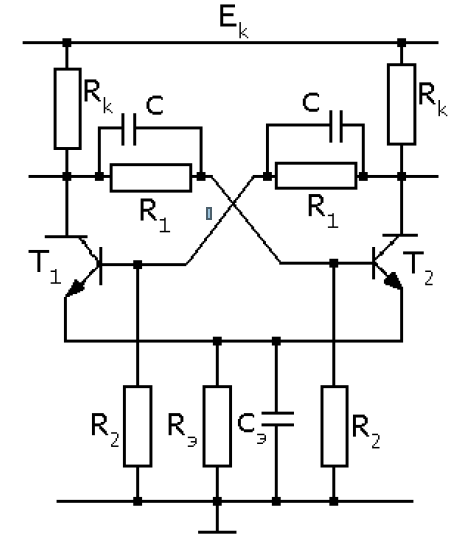
\includegraphics{image/screenshot001}
	\caption{Триггер с автоматическим смещением.}
	\label{fig:screenshot001}
\end{figure}

Рассмотрим схему симметричного триггера (см рис. 1). Триггер представляет собой
два усилителя на транзисторах Т1 и Т2. Выход одного усилителя соединен со входом
другого и наоборот. Таким образам образуется положительная обратная связь.

В принципе в такой схеме возможно состояние, когда оба транзистора открыты и
пребывают в равновесии, однако на практике малейшая флуктуация тока или напряжения
приведет к лавинообразному процессу закрытия одного транзистору и еще большему
открытию другого.

Если параметры схемы выбраны так, что когда один из транзисторов закрыт, другой
открыт и насыщен, то такой триггер называют насыщенным. Если открытый транзистор
находится на границе активной области, то такой триггер называют ненасыщенным.

В одном из устойчивых состояний триггер может находиться сколь угодно долго,
пока не поступит управляющий сигнал. Пусть он поступает на базу запертого транзистора
Т2. Как только напряжение на базе Т2 достигнет уровня отпирания появится коллекторный
ток Iб2 и, следовательно, уменьшится ток базы Iб1. Т1 выйдет в активную область и будет
восстановлена петля обратной связи. Возникающий при этом регенеративный процесс
аналогичен описанному выше. В итоге Т1 закроется, а Т2 откроется и окажется в области
насыщения. Триггер переедет в другое устойчивое состояние.

Конденсаторы включены для ускорения процесса переключения и называются
ускоряющими. Они также обеспечивают четкость процесса переключения.

\begin{figure}[H]
	\centering
	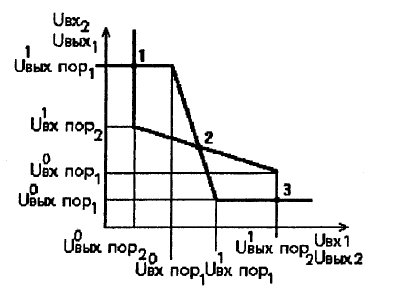
\includegraphics{image/screenshot002}
	\caption{Передаточная характеристика}
	\label{fig:screenshot002}
\end{figure}

Процесс переключения триггера удобно описывать с помощью передаточных
характеристик (см рис.). Состояния равновесия находятся в точках пересечения
передаточных характеристик (1,2, 3), причем точка 2 не является устойчивой (см. выше).

Пусть на вход 1 подан запирающий сигнал. Процесс переключения триггера можно
разбить на несколько этапов (см. рис. 3):

Стадия подготовки начинается в момент подачи на вход импульса и включает в себя
время рассасывания избыточных носителей в базе Т1 (tР) и формирования на коллекторе Т1
отрицательного фронта (tП), на котором Т1 работает уже в активном режиме и ток IK1
уменьшается а UK1 растет. Этот перепад напряжения передается через конденсатор на базу
Т2 и, когда потенциал Uб2 компенсирует начальное смещение, транзистор Т2 открывается.

Стадия регенерации (tРЕГ) начинается с отпирания Т2, после чего в течение
некоторого времени открыты оба транзистора. На этой стадии приращение коллекторных
токов почти полностью идет в базу противоположного транзистора через С, что ускоряет
переходный процесс.

Затем следует стадия динамической отсечки, на которой процессы идут в прежнем
направлении, но с меньшей скоростью, хотя VТ1 уже не управляем.

Стадия восстановления начинается с запирания Т1 и продолжается до установления
устойчивого состояния. Она состоит из трех этапов: формирования положительного фронта
на коллекторе Т2 (tФ+), отрицательного фронта на коллекторе Т1 (tФ-), и этапа динамического
смещения (tД.С.), на котором потенциал базы закрывшегося Т1 уменьшается до статического
Uб0.

\subsection{Функциональные типы триггеров.}

В зависимости от комбинации управляющих сигналов, вызывающих изменение
состояния, триггеры подразделяются на несколько функциональных типов. Тип триггера
определяется по таблице состояний, которая указывает значение выходного сигнала Qn+1
после переключения триггера (в момент времени tn+1) в зависимости от значений
управляющих сигналов и выходного сигнала Qn до переключения (в момент времени tn). В
данной лабораторной работе рассматриваются RS триггеры и Т триггеры.

RS триггеры имеют 2 входа S и R. При подаче логических нулей на оба входа триггер
сохраняет своё предыдущее состояние, при подаче логической единицы на вход S триггер
переходит в единичное состояние (или остается в таковом), при подаче логической единицы
на вход R триггер переходит в нулевое состояние (или остается в таковом), при подаче
логической единицы на оба входа триггер оказывается в неопределенном состоянии – такая
комбинация входных сигналов является запрещенной.

\begin{table}[H]
	\begin{center}
		\tablecaption{Таблица состояний RS триггера}
	\begin{tabular}{|c|c|c|}
		\hline
		R & S & $Q^{n+1}$  \\ \hline
		0 & 0 & $Q^n$  \\ \hline
		0 & 1 & 1 \\ \hline
		1 & 0 & 0 \\ \hline
		1 & 1 & X \\ \hline
	\end{tabular}
	\end{center}
\end{table}

Схема RS триггера представлена на рис. 2. Пусть входом S является точка 4, а входом
R является точка 14, тогда выходом Q является точка 13, а выходом Q является точка 3.

Пусть на вход S подана логическая единица US=U1 (высокий потенциал), а на вход R -
логический ноль UR =U0 (низкий потенциал); тогда транзистор T1 – насыщен, а Т4 – в
отсечке. Следовательно, потенциал выхода Q низкий: UK1 =UK2 = 0
Q
U U   , эта точка цепью
обратной связи R4 – C1 соединена с базой транзистора Т3, следовательно, потенциал UБ3 –
низкий, и Т3 – заперт (в отсечке); благодаря этому, потенциал выхода Q высокий:
1
K3 K 4 Q U U U U , эта точка цепью обратной связи R8 – C2 соединена с базой транзистора
Т2, следовательно, потенциал UБ2 – высокий, и Т2 – насыщен; благодаря этому, потенциал
выхода Q низкий 0
K1 K 2
Q
U U U U     . Если теперь на вход S подать логический ноль US=U0
и на вход R – по-прежнему логический ноль UR =U0, то транзистор Т1 запрется, а транзистор
Т2 останется насыщенным, т.е. триггер останется в единичном состоянии.

Пусть на вход S подан логический ноль US=U0 (низкий потенциал), а на вход R -
логическая единица UR =U1 (высокий потенциал); тогда транзистор T1 – заперт (в отсечке), а
Т4 – насыщен. Следовательно, потенциал выхода Q низкий: UK3 =UK4 = 0
Q U U , эта точка
цепью обратной связи R8 – C2 соединена с базой транзистора Т2, следовательно, потенциал
UБ2 – низкий, и Т2 – заперт (в отсечке); благодаря этому, потенциал выхода Q высокий:
1
K1 K 2 Q U U U U , эта точка цепью обратной связи R4 – C1 соединена с базой транзистора
Т3, следовательно, потенциал UБ3 – высокий, и Т3 – насыщен; благодаря этому, потенциал
выхода Q низкий 0
K3 K 4 Q U U U U . Если теперь на вход R подать логический ноль
UR=U0 и на вход S – по-прежнему логический ноль US =U0, то транзистор Т4 запрется, а
транзистор Т3 останется насыщенным, т.е. триггер останется в нулевом состоянии.

Пусть на оба входа подан высокий потенциал логической единицы US = UR = U1, тогда
оба входных транзистора Т4 и Т1 – открыты (в нормальном активном режиме), в каком
состоянии окажется триггер после окончания входных сигналов непонятно, следовательно
это – запрещенная комбинация входных сигналов.

Т-триггеры (счетные триггеры) имеют один вход Т (счетный вход). При подаче
логического нуля на вход триггер сохраняет своё предыдущее состояние, при подаче
логической единицы на вход триггер меняет свое состояние.

\begin{table}[H]
	\begin{center}
		\tablecaption{Таблица состояний Т триггера}
		\begin{tabular}{|c|c|}
			\hline
			T & $Q^{n}$  \\ \hline
			0 & $Q^{n+1}$  \\ \hline
			1 & $\overline{Q^{n}}$ \\ \hline
		\end{tabular}
	\end{center}
\end{table}

Управляющая цепь Т-триггера состоит из трех диодов D1,D2,D3 и конденсатора CBX,
см. рис. 4.

Пусть Т1 насыщен, а Т2 в отсечке, т.е. триггер находится в единичном состоянии,
тогда на базе Т1 и на катоде D1 высокий потенциал, а на базе Т2 и на катоде D2 низкий.
Следовательно, диод D1 заперт, а диод D2 вблизи точки открывания. При подаче на вход
положительного импульса D1 остается закрытым, а D2 открывается и пропускает
положительный импульс на базу Т2, который переходит в насыщение и, тем самым, триггер
переходит в нулевое состояние. Теперь D1 будет приоткрыт, а D2 заперт и следующий
положительный импульс будет насыщать Т1, переводя триггер в единицу.

\section{Описание установки}

Работа выполняется на стенде в лаборатории микроэлектроники на блоке № 132.

На стенде кроме прочего имеются:

\begin{itemize}
	\item Блок для изучения симметричного триггера с двумя биполярными транзисторами в
	каждом плече.
	\item Блок питания с двумя регулируемыми источниками постоянного напряжения
	-6...+6 В и нерегулируемыми источниками постоянного напряжения +5 В, +6.3 В, +12 В.
\end{itemize}

В состав установки также входят:

\begin{itemize}
	\item Три цифровых мультиметра для измерения постоянных напряжений и тока в
	первой части работы.
	\item Генератор сигналов прямоугольной формы (генератор импульсов).
	\item Осциллограф.
\end{itemize}

На стенде собрана одна из схем симметричного триггера — схема с автоматическим
смещением. Главным достоинством этой схемы является наличие только одного источника
питания и высокая стабильность по отношению к изменению напряжения питания. К числу
его недостатков можно отнести следующие:

\begin{itemize}
	\item выходное напряжение триггера на величину URЭ меньше, чем при постороннем смещении
	(RЭ=R6);
	\item минимальный потенциал коллектора (при насыщении транзистора) не равен нулю, а
	составляет величину URЭ
	\item схема требует двух дополнительных элементов: RЭ и СЭ, причем емкость СЭ весьма
	большая, а сопротивление RЭ бесполезно расходует мощность до 10\% от всей рассеиваемой
	мощности.
\end{itemize}

Отметим некоторые особенности этой схемы. Роль э.д.с. смещения базы здесь играет
падение напряжения на RЭ, равное потенциалу насыщенного транзистора Ut. Если считать
насыщенный транзистор одним узлом, то этот потенциал можно найти по формуле:

$$U_t = \dfrac{U_{pit} * (\dfrac{1}{R_9} + \dfrac{1}{R_9 + R_8})}{\dfrac{1}{R_9} + \dfrac{1}{R_9 + R_8} + \dfrac{1}{R_7} + \dfrac{1}{R_8 + R_7} \dfrac{1}{R_6}}$$

Повышенная стабильность данной схемы объясняется тем, что напряжение смещения
Ut пропорционально ЕПИТ, тогда как в обычной схеме э,д.с. ЕБ и ЕПИТ независимы и при
изменении одного из них нарушилась бы равновесие обратной связи. Работоспособность же
такой схемы не ухудшается вплоть до ЕПИТ1В, однако при снижении ЕПИТ снижается и
выходное напряжение.

В схему дополнительно введено по два транзистора в каждое плечо (VТ1 и VТ4) для
работы в качестве управляющих.

Ниже описано назначение клемм, имеющихся на стенде:

4, 14 — вход левого и правого плеча соответственно;

7, 8 — контакты базы транзисторов обратной связи обоих плечей;

3, 13 — выходы;

5, 6 — клеммы, замыкаемые при подключении ускоряющего конденсатора;

12 — контакт питания + 12В;

0 — земля.

\section{Результаты измерений}

\begin{table}[H]
	\begin{center}
		\tablecaption{Таблица состояний Т триггера}
	\begin{tabular}{|l|l|l|l|l|l|l|l|}
		\hline
		&         & V3    & V13   & V6   & V7   & V10  & Ir, mA \\ \hline
		Q=1 & S=1 R=0 & 2.3   & 11.19 & 0.7  & 2.9  & 2.2  & 0.818  \\ \hline
		& S=0 R=0 & 2.1   & 11.18 & 0.7  & 2.7  & 2    & 0.833  \\ \hline
		Q=0 & S=0 R=1 & 11    & 2.57  & 3.2  & 0.9  & 2.5  & 0.166  \\ \hline
		& S=0 R=0 & 11.04 & 2.47  & 3.06 & 0.86 & 2.34 & 0.159  \\ \hline
		& S=1 R=1 & 3.84  & 3.83  & 1.26 & 1.33 & 3.77 & 0.247  \\ \hline
	\end{tabular}
\end{center}
\end{table}



\section{Вычисление параметров модели}

\section{Схемы расчета ВАХ}

\section{Графики ВАХ}


\end{document} % конец документа